The form of most molecular mechanics energy potentials is reasonably consistent, following the general form of equation \ref{equation:opls}.
\begin{equation}
E \left(r^N \right ) = E_\mathrm{bonds} + E_\mathrm{angles} + E_\mathrm{dihedrals} + E_\mathrm{nonbonded}
\label{equation:opls}
\end{equation}

Bonds and angles are modeled as springs and dihedrals as a Fourier series, as shown in equations below.
\begin{equation}
E_\mathrm{bonds} = \sum_\mathrm{bonds} K_r (r-r_0)^2
\end{equation}

\begin{equation}
E_\mathrm{angles} = \sum_\mathrm{angles} k_\theta (\theta-\theta_0)^2
\end{equation}

\begin{equation}
E_\mathrm{dihedrals} = \sum_{i=1\dots4} {\frac {V_i} {2} \left [ 1 + \cos \left ( i * (\phi-\phi_0) \right ) \right ] }
\end{equation}

The non-bonded terms are modeled as a Columbic potential between any point charges and a Lennard-Jones or 6-12 potential between any non-bonded atoms (equation \ref{equation:nonbonded}).
These non-bonded atoms are phased in by a ``fudge factor'' for atoms in a 1-4 configuration.
\begin{equation}
\begin{split}
E_\mathrm{nonbonded} = \sum_{i>j} f_{ij} 
                \left (
                        \frac {q_i q_j e^2}{r_{ij}}
                    + 4 \epsilon_{ij} 
                    \left  [  
                        \left ( \frac{\sigma_{ij}}{r_{ij}}\right )^{12}
                      - \left ( \frac{\sigma_{ij}}{r_{ij}}\right )^{6}
                    \right ]
                \right )
\\
f_{ij} = 
  \begin{dcases*}
   0    & if $i$ and $j$ are separated by 2 or fewer bonds\\
   0.5  & if $i$ and $j$ are separated by 3 bonds\\
   1.0  & otherwise
  \end{dcases*}
\end{split}
\end{equation}

Where $\sigma_{ij} = \sqrt{\sigma_{ii} \sigma_{jj}}$ and $\epsilon_{ij} = \sqrt{\epsilon_{ii}\epsilon_{jj}}$ \cite{jorgensen1996development}.
The terms of the energy model are illustrated in figure \ref{figure:force_field}.

\begin{figure}
\centering
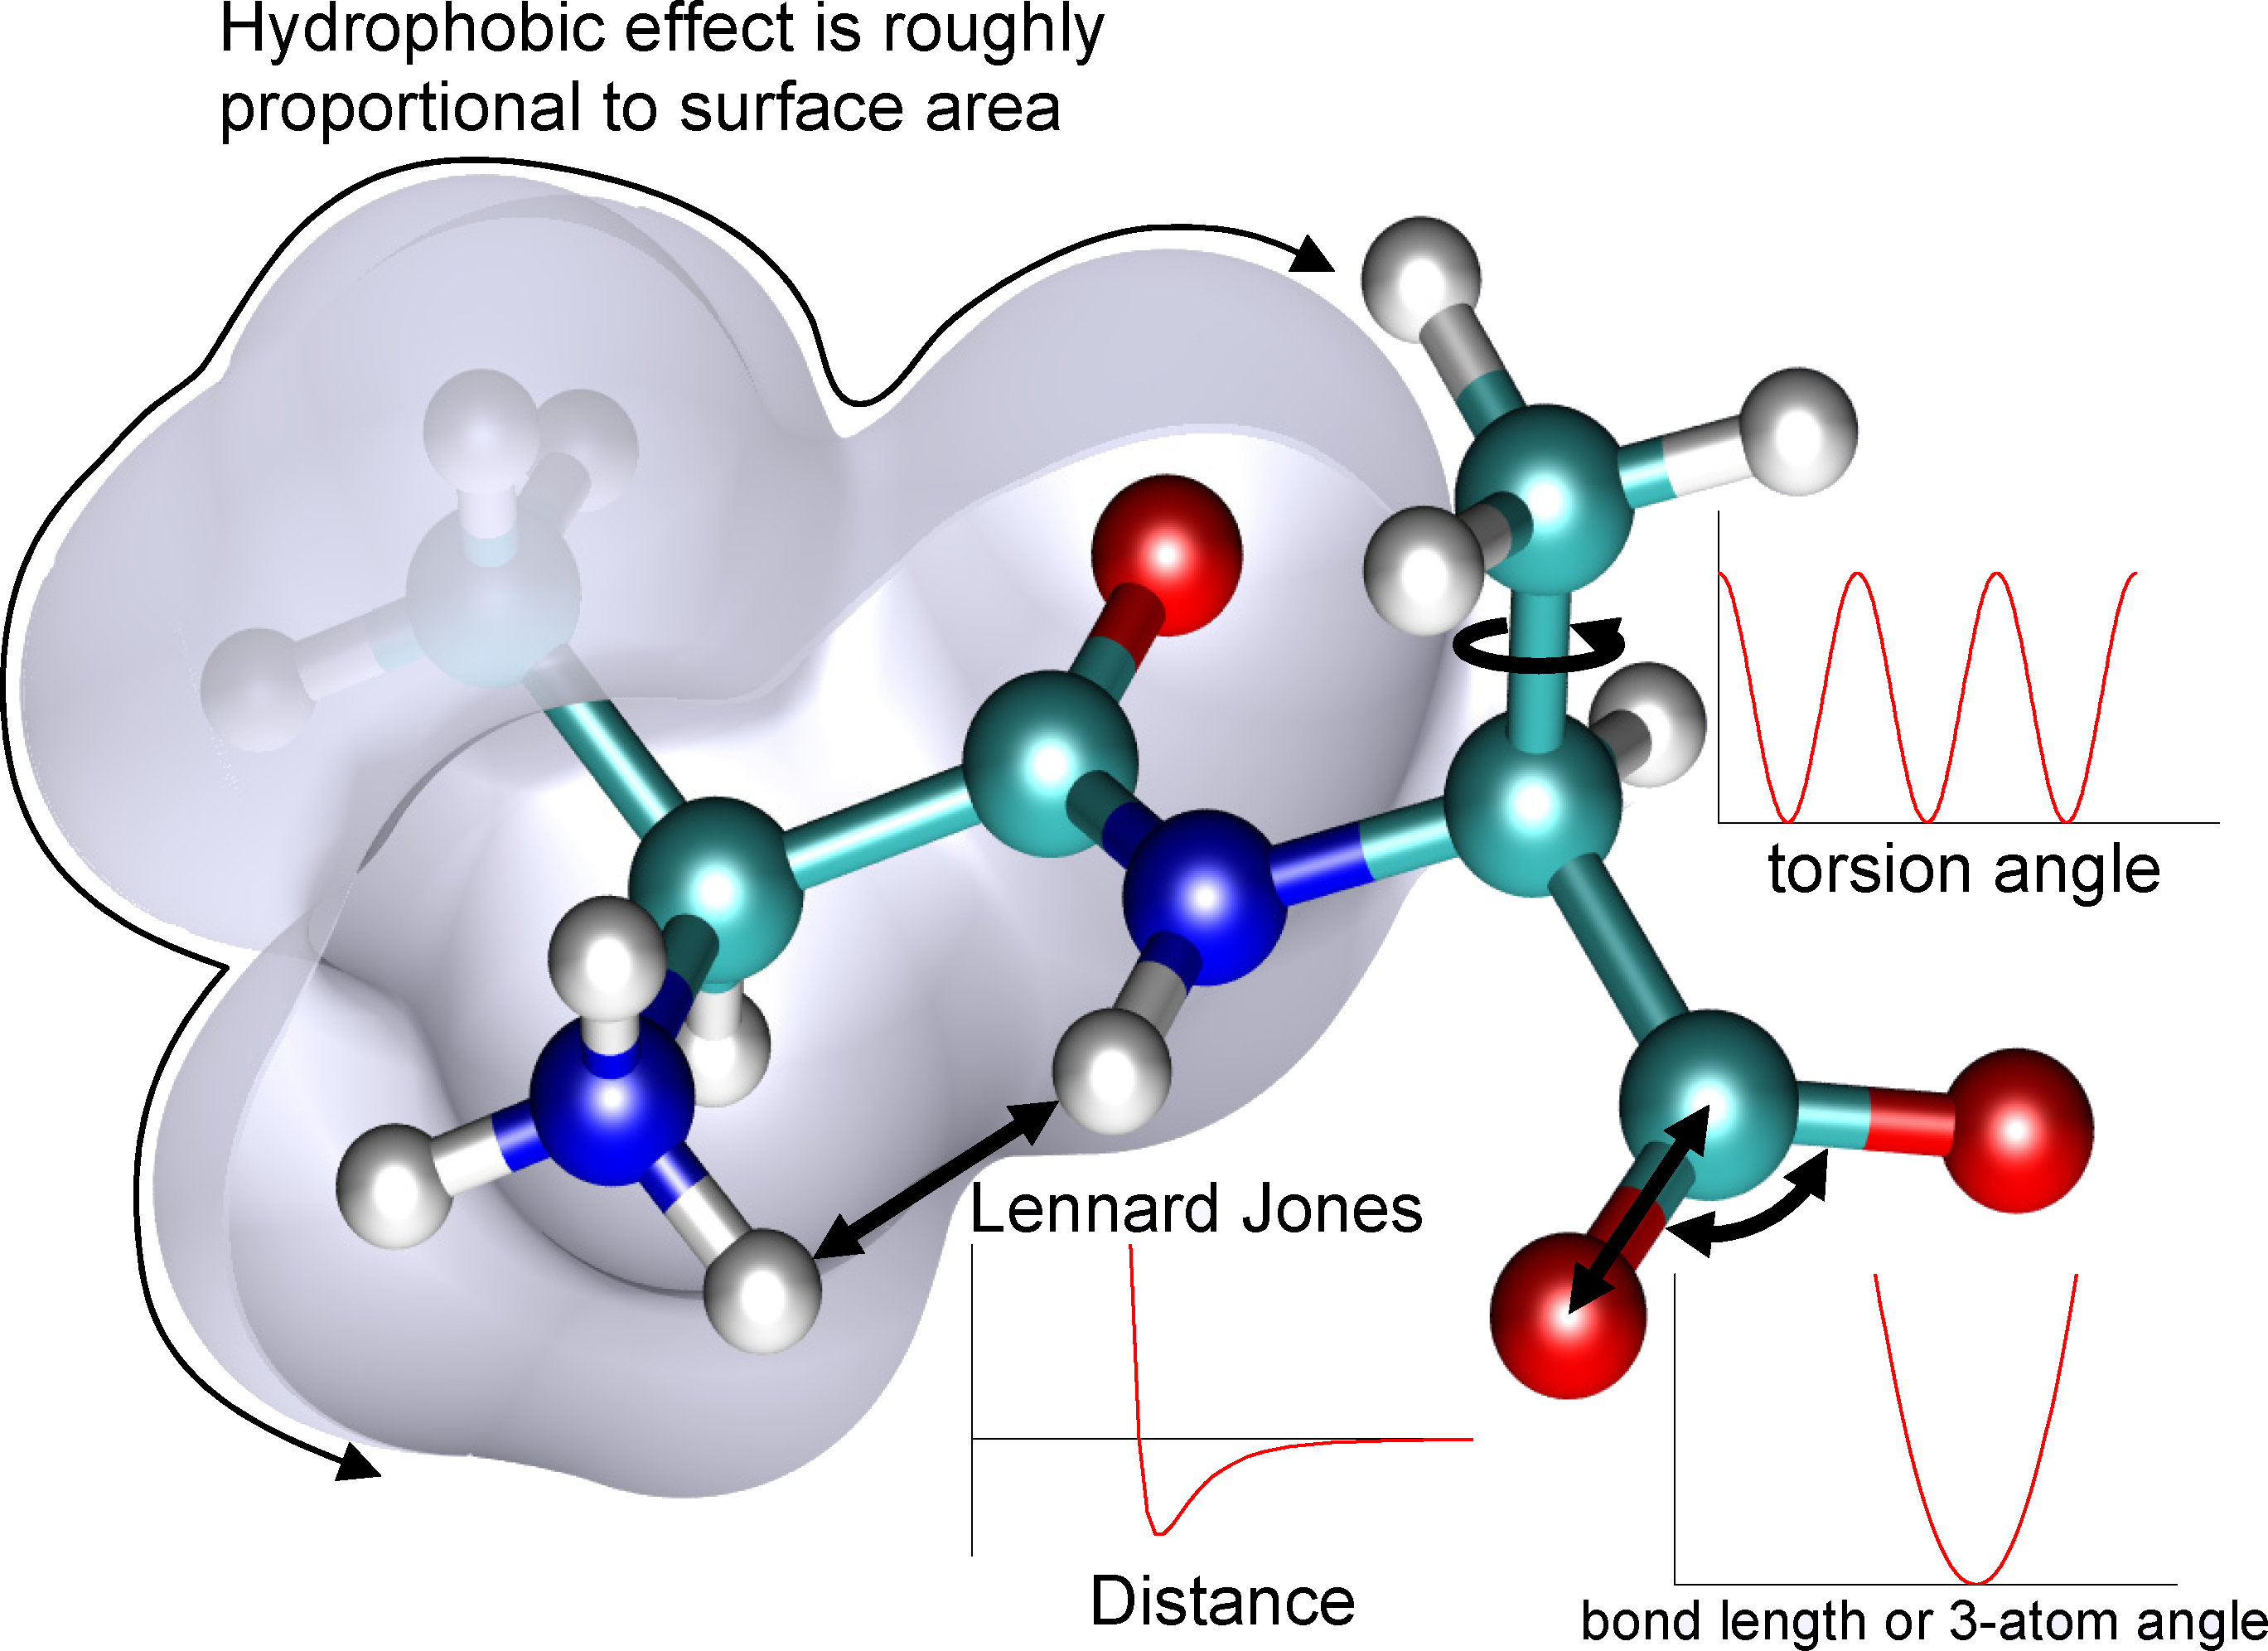
\includegraphics[width=0.8\textwidth,height=0.8\textwidth,keepaspectratio]{figures/molecular_mechanics_force_field2.png}
\caption{A molecule illustrating some of the major terms present in molecular mechanics force fields.
Figure adapted from \protect\cite{boas2007potential}, and licensed under cc-by-sa 3.0 license.}
\label{figure:force_field}
\end{figure}

Energy models following this form have a number of desirable characteristics.
First, they are reasonably accurate, having been shown to accurately predict a number of different physical phenomena.
Second, they are significantly less expensive to compute than quantum mechanical energy formulations.
Third, because the terms of the energy model are differentiable, using this form of an energy model is conducive to using one of the minimization techniques discussed in \nameref{subsection:minimization} (\ref{subsection:minimization}).
